\subsection{M.PC.11 - Rischi inattesi}
\begin{figure}[H]
    \centering
    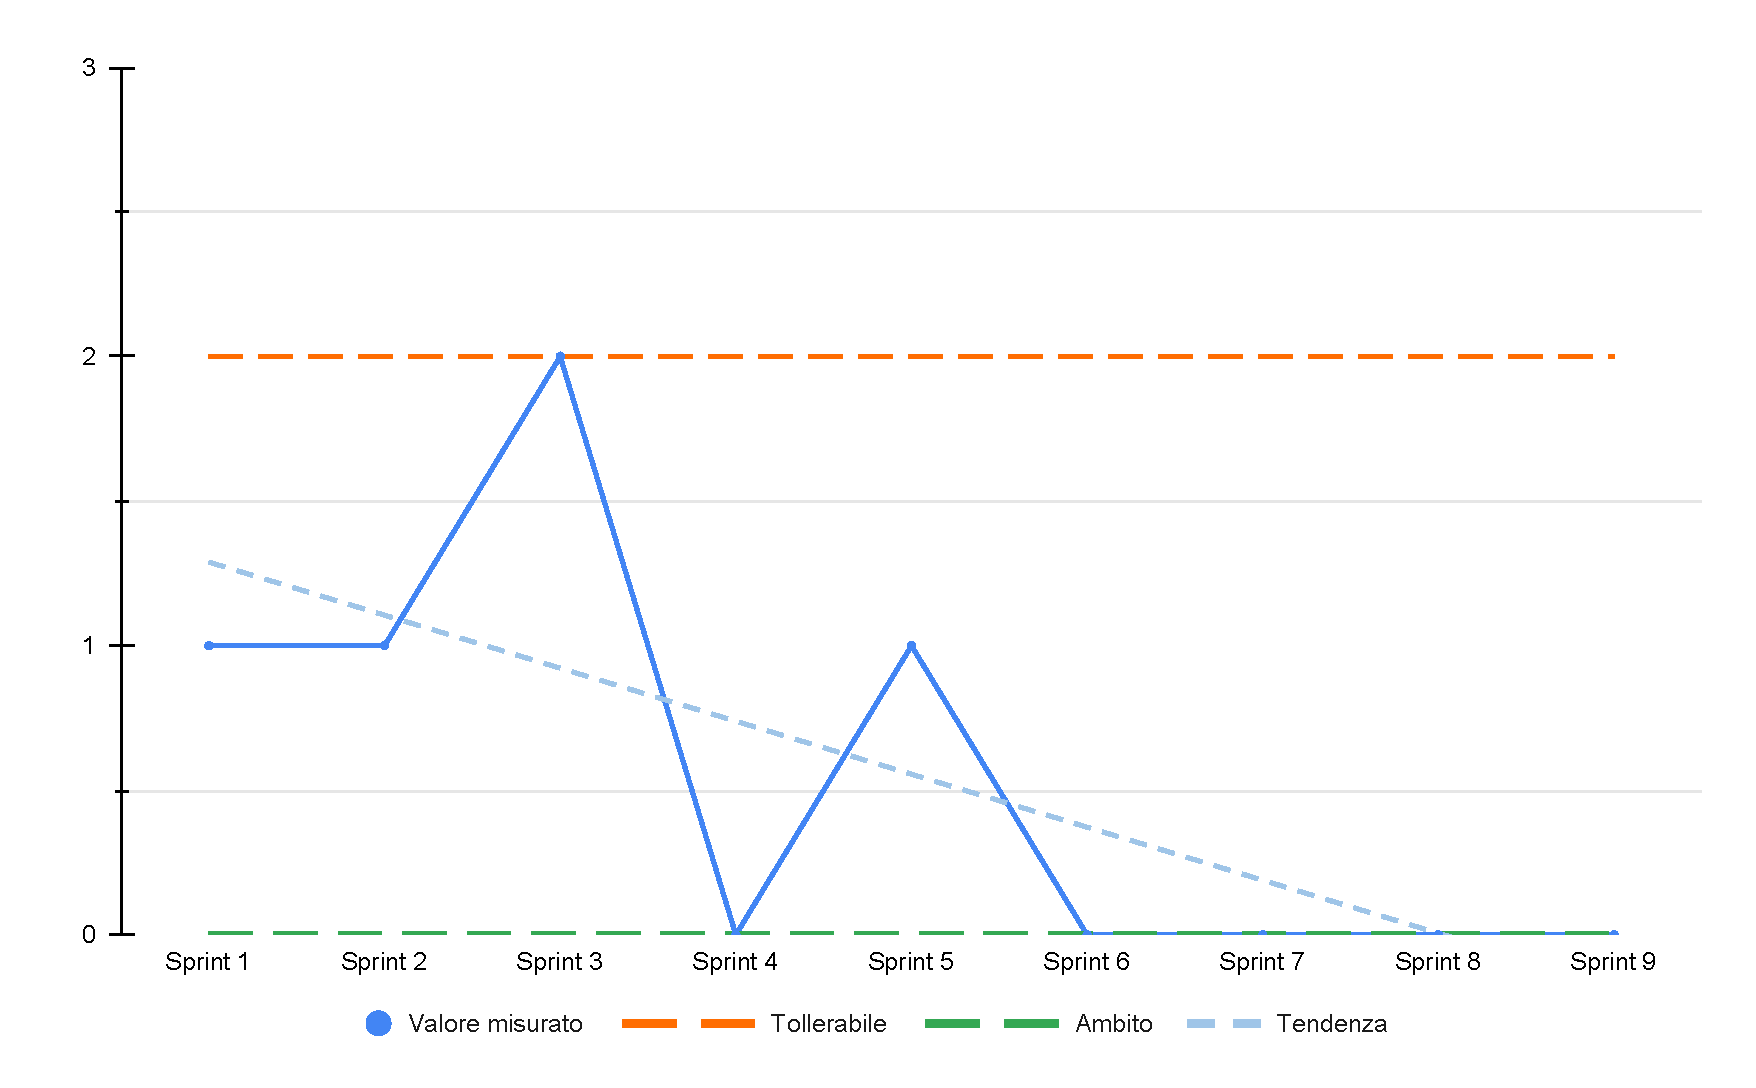
\includegraphics[width=\textwidth]{assets/rischi_inattesi.pdf}
    \caption{M.PC.11 - Rischi inattesi}
\end{figure}

\par Il grafico evidenzia l’inesperienza iniziale del team nell’individuare i rischi che possono emergere durante lo svolgimento di un progetto software. Nei primi tre \glossario{sprint}, infatti, il gruppo ha dovuto affrontare almeno un rischio inatteso. Ciononostante, il numero di rischi imprevisti è rimasto entro i limiti della soglia tollerabile. A partire dal quarto sprint, i rischi che si sono verificati erano già stati analizzati e documentati nel \PdP. Attraverso un’analisi più consapevole, una collaborazione stretta tra i membri e una comunicazione trasparente, il team ha mantenuto il numero di eventi imprevisti stabile e prossimo al valore ambito. L'unica eccezione è stata il sesto sprint, durante il quale è emerso un rischio inatteso legato al cambio di tecnologie. Nonostante il gruppo avesse previsto una possibile transizione e avesse testato diversi \glossario{framework} alternativi, l’entità del lavoro risultante ha superato le risorse disponibili, prolungando le scadenze prefissate. Per migliorare la gestione del progetto, il gruppo ha convenuto di discutere e monitorare i rischi durante le riunioni interne, fornendo al responsabile una base solida per la stesura del \PdP. L'obiettivo per le iterazioni successive è ridurre il valore tollerabile a 1, al fine di mantenere una gestione stabile dei rischi.
